\documentclass[class={IEEEtran}]{standalone}
\usepackage{fontawesome7}
\usepackage{tikz}
\usepackage{amsmath}
\usepackage{pgf}
\usepackage{pifont}
\usepackage{xcolor}
\usepackage{contour}
\usepackage{mathptmx}

\contourlength{1pt} 
\pagestyle{empty}
\usetikzlibrary{shapes.geometric,shapes.arrows,positioning,calc,arrows.meta,math,backgrounds}

% --------- DEFINE COLORS ---------
% Blue 系
\definecolor{blue}{RGB}{76,114,176}        % 沉稳学术蓝
\definecolor{navy}{RGB}{59,72,99}           % 深藏青
\definecolor{steelblue}{RGB}{102,139,171}   % 钢蓝

% Red 系
\definecolor{red}{RGB}{180,82,82}           % 暗红（非警告型）
\definecolor{maroon}{RGB}{128,70,70}        % 学术酒红
\definecolor{brick}{RGB}{150,90,75}         % 砖红

% Green 系
\definecolor{green}{RGB}{90,140,120}        % 灰绿色
\definecolor{olive}{RGB}{120,130,90}        % 橄榄绿
\definecolor{forest}{RGB}{80,110,95}        % 深林绿

% Yellow / Orange 系
\definecolor{orange}{RGB}{200,140,90}       % 低饱和橙
\definecolor{goldenrod}{RGB}{170,145,85}    % 学术金
\definecolor{sand}{RGB}{190,175,140}        % 沙色

% Purple 系
\definecolor{purple}{RGB}{130,110,150}      % 灰紫
\definecolor{plum}{RGB}{120,95,125}         % 李子紫
\definecolor{violet}{RGB}{145,130,170}      % 冷紫

% Gray 系（强烈推荐学术使用）
\definecolor{gray}{RGB}{130,130,130}
\definecolor{darkgray}{RGB}{90,90,90}
\definecolor{lightgray}{RGB}{200,200,200}
% ---------------------------------
% ---- DEFINE GLOBAL VARIABLES ----
\newcommand{\AGENTSPAN}{0.2\textwidth}
\newcommand{\LINEHEIGHT}{3.2ex}
\newcommand{\ENDWIDTH}{1.4em}
\newcommand{\ENDHEIGHT}{0.4ex}
\newcommand{\LABELSIZE}{1}
\newcommand{\LABELCOLOR}{black}
% ---------------------------------
% --------- DEFINE STYLES ---------
\tikzset{AGENT/.style={rectangle,minimum width=5em,minimum height=3.5ex,draw,semithick,align=flush center, anchor=north,fill=white}}
\tikzset{ACTION/.style={rectangle,rounded corners,draw,semithick,align=flush left,fill=white}, anchor=north}
\tikzset{LABEL/.style={circle, draw, semithick, align=center, minimum size=1.2em, inner sep=0pt,fill=white}, anchor=north}
\tikzset{PREPARATION/.style={rectangle,draw,semithick,align=flush center,fill=white,dashed, anchor=north}}

% 基础单向箭头
\tikzset{Arrow/.style={thick, -stealth}}
% 基础单向箭头（细）
\tikzset{ArrowThin/.style={->,>=stealth, thin}}
% 加粗单向箭头
\tikzset{ArrowThick/.style={->,>=stealth, very thick}}
% 虚线箭头（流程/假设）
\tikzset{ArrowDash/.style={->,>=stealth, dashed, thick}}
% 点线箭头（弱关系）
\tikzset{ArrowDot/.style={->,>=stealth, dotted, thick}}
% 双向箭头
\tikzset{BiArrow/.style={<->,>=latex, thick}}
% 超粗双向箭头（强调用）
\tikzset{BiArrowThick/.style={<->,>=latex, very thick}}

\tikzset{LineThin/.style={thin}}
\tikzset{LineThick/.style={thick}}
\tikzset{LineDashed/.style={dashed, thin}}
\tikzset{LineDotted/.style={dotted, thick}}
% ---------------------------------
% -------- DEFINE COMMANDS --------
\newcommand{\NewCoord}[2]{\coordinate (#1) at (#2)}
\newcommand{\NewCoordRightToC}[3]{\coordinate (#1) at ($(#2)+(#3,0)$)}
\newcommand{\NewCoordBelowToC}[3]{\coordinate (#1) at ($(#2)+(0,-#3)$)}
\newcommand{\NewCoordRightToN}[3]{\coordinate (#1) at ($(#2.east |- #2.north)+(#3,0)$)}
\newcommand{\NewCoordBelowToN}[3]{\coordinate (#1) at ($(#2.south)+(0,-#3)$)}
\newcommand{\NewCoordAlignToN}[3]{\coordinate (#1) at ($(#3 -| #2.north)$)}

\newcommand{\NewNode}[4]{\node[#1] (#2) at (#3) {#4}}
\newcommand{\NewAgent}[3]{\node[AGENT] (#1) at (#2) {#3}}
\newcommand{\NewAction}[3]{\node[ACTION] (#1) at (#2) {#3}}
\newcommand{\NewLabel}[3]{\node[LABEL, scale=\LABELSIZE, text=\LABELCOLOR, draw=\LABELCOLOR] (#1) at (#2) {#3}}

\newcommand{\DrawLine}[3]{\draw[#1] (#2) -- (#3)}
\newcommand{\DrawArrow}[4]{\draw[#1] (#2) -- (#3) node[midway,above=-3pt]{\contour{white}{#4}}}

\makeatletter
\newcommand{\GetLowestCoord}[2]{%
    \global\pgf@ya=999pt%
    \def\pgf@lowest{(0,0)}%
    \foreach \p in {#2} {%
        \pgfextracty{\pgf@yb}{\pgfpointanchor{\p}{center}}%
        \ifdim\pgf@yb<\pgf@ya
          \global\pgf@ya=\pgf@yb
          \xdef\pgf@lowest{\p}%
        \fi
    }%
    \coordinate (#1) at (\pgf@lowest)
}
\makeatother

\newcommand{\DrawEnd}[2] {
  \NewCoordBelowToC{end_#1}{#2-|#1}{\LINEHEIGHT/2};
  \draw[semithick] (#1.south) -- (end_#1);
  \draw[fill=black] ($(end_#1)+(-\ENDWIDTH,0)$) rectangle ($(end_#1)+(\ENDWIDTH,-\ENDHEIGHT)$);
}
% ---------------------------------

\renewcommand{\AGENTSPAN}{0.18\textwidth}
\newcommand{\COMMONCOLOR}{gray}
\newcommand{\SPECIALCOLOR}{black}

\begin{document}
\begin{tikzpicture}

% ========================================
%   Agents
% ========================================
\NewCoord{c_MF}{0,0};
\NewAgent{agent_MF}{c_MF}{\hspace{-0.5em} \faBasketShopping \; MF};

\NewCoordRightToC{c_MS}{c_MF}{\AGENTSPAN};
\NewAgent{agent_MS}{c_MS}{\hspace{-0.5em} \faServer \; MS};

\NewCoordRightToC{c_PS}{c_MS}{\AGENTSPAN};
\NewAgent{agent_PS}{c_PS}{\hspace{-0.5em} \faSackDollar \; PS};

% ========================================
%   Messages
% ========================================

% Phase 2: Prepayment
% -------------- Divide Line --------------
  \NewCoordRightToC{c_tmp}{agent_MF.south}{-0.06\textwidth};
  \NewCoordBelowToC{c_ldiv_2}{c_tmp}{\LINEHEIGHT/3};
  \NewCoordAlignToN{c_tmp}{agent_PS}{c_ldiv_2};
  \NewCoordRightToC{c_rdiv_2}{c_tmp}{0.06\textwidth};
  \DrawLine{LineDotted}{c_ldiv_2}{c_rdiv_2};
% ----------------------------------------
% ---------------- Label -----------------
  \renewcommand{\LABELSIZE}{1}
  \renewcommand{\LABELCOLOR}{black}
  \NewCoordBelowToC{c_tmp}{c_ldiv_2}{\LINEHEIGHT*2.9};
  \NewCoordRightToC{c_label_2}{c_tmp}{1em};
  \NewLabel{label_2}{c_label_2}{\romannumeral 2};
% ----------------------------------------

\NewCoordBelowToC{c_act_MS1}{c_ldiv_2-|c_MS}{\LINEHEIGHT/2};
\NewNode{ACTION, draw=\SPECIALCOLOR}{action_MS1}{c_act_MS1}{
  $id_{order} := random()$\\
  $amount, description := caculate(goods)$\\
  $order = id_{M} || id_{order} || amount || description$\\
  $S_{order} := sign_{priv_{M}}(order)$
};

\NewCoordBelowToN{c_smsg_MS_PS_2}{action_MS1}{\LINEHEIGHT};
\NewCoordAlignToN{c_rmsg_MS_PS_2}{agent_PS}{c_smsg_MS_PS_2};
\DrawArrow{Arrow, color=\SPECIALCOLOR}{c_smsg_MS_PS_2}{c_rmsg_MS_PS_2}{$order, S_{order}$};

\NewCoordBelowToC{c_act_PS1}{c_rmsg_MS_PS_2}{\LINEHEIGHT/2};
\NewNode{ACTION, draw=\SPECIALCOLOR}{action_PS1}{c_act_PS1}{
  \textbf{if} $verify(S_{order})$ \textbf{then} \\
  \quad $id_{prepay} := random()$\\
  \quad $store(id_{prepay}, order)$\\
  \textbf{else} $abort()$
};

\NewCoordBelowToN{c_smsg_PS_MS_1}{action_PS1}{\LINEHEIGHT};
\NewCoordAlignToN{c_rmsg_PS_MS_1}{agent_MS}{c_smsg_PS_MS_1};
\DrawArrow{Arrow, color=\SPECIALCOLOR}{c_smsg_PS_MS_1}{c_rmsg_PS_MS_1}{$id_{prepay}$};

\NewCoordBelowToC{c_act_MS_2}{c_rmsg_PS_MS_1}{\LINEHEIGHT/2};
\NewNode{ACTION, draw=\SPECIALCOLOR}{action_MS2}{c_act_MS_2}{
  $S_{prepay} := sign_{priv_{M}}(id_{prepay} || id_{M})$\\
  $params := id_{prepay} || id_{M} || S_{prepay}$
};

\NewCoordBelowToN{c_smsg_MS_MF_1}{action_MS2}{\LINEHEIGHT};
\NewCoordAlignToN{c_rmsg_MS_MF_1}{agent_MF}{c_smsg_MS_MF_1};
\DrawArrow{Arrow}{c_smsg_MS_MF_1}{c_rmsg_MS_MF_1}{$params$};

\NewCoordBelowToC{c_smsg_MF_PS_1}{c_rmsg_MS_MF_1}{\LINEHEIGHT};
\NewCoordAlignToN{c_rmsg_MF_PS_1}{agent_PS}{c_smsg_MF_PS_1};
\DrawArrow{Arrow}{c_smsg_MF_PS_1}{c_rmsg_MF_PS_1}{$params$};

\NewCoordBelowToC{c_act_PS1}{c_rmsg_MF_PS_1}{\LINEHEIGHT/2};
\NewNode{ACTION, draw=\SPECIALCOLOR}{action_PS1}{c_act_PS1}{
  \textbf{if} $verify(S_{prepay})$ \\
  \textbf{then} $continue()$\\
  \textbf{else} $abort()$
};

% Phase 3: Payment
% -------------- Divide Line --------------
  \NewCoord{c_tmp}{action_PS1.south -| c_ldiv_2};
  \NewCoordBelowToC{c_ldiv_3}{c_tmp}{\LINEHEIGHT/2};
  \NewCoordAlignToN{c_tmp}{agent_PS}{c_ldiv_3};
  \NewCoordRightToC{c_rdiv_3}{c_tmp}{0.06\textwidth};
  \DrawLine{LineDotted}{c_ldiv_3}{c_rdiv_3};
% ----------------------------------------

% ========================================
%   Ends
% ========================================
\begin{scope}[on background layer]
  \GetLowestCoord{c_lowest}{c_rdiv_3};
  \DrawEnd{agent_MF}{c_lowest};
  \DrawEnd{agent_MS}{c_lowest};
  \DrawEnd{agent_PS}{c_lowest};
\end{scope}

\end{tikzpicture}
\end{document}
